% CREATED BY MAGNUS GUSTAVER, 2020
\chapter{Theory} \label{Theory}
This section presents theory used in this thesis. It starts with the hardware used to
enable autonomous flight of the drone, then the software and how communication between the computer the phone is handled. 


\todo{Se till att theory INTE innehåller någofn form av implementation, det som står i theory ska presentera den hård- och mjukvara som vi får tilldelat samt deras begränsingar}



\section{Hardware} \label{Hardware}
In this section the hardware that is used will be presented, which is a drone, a mobile device and the test objects. 

\subsection{DJI mavic 2 enterprise zoom} \label{DJI}


\begin{figure}[h!]
\centering
 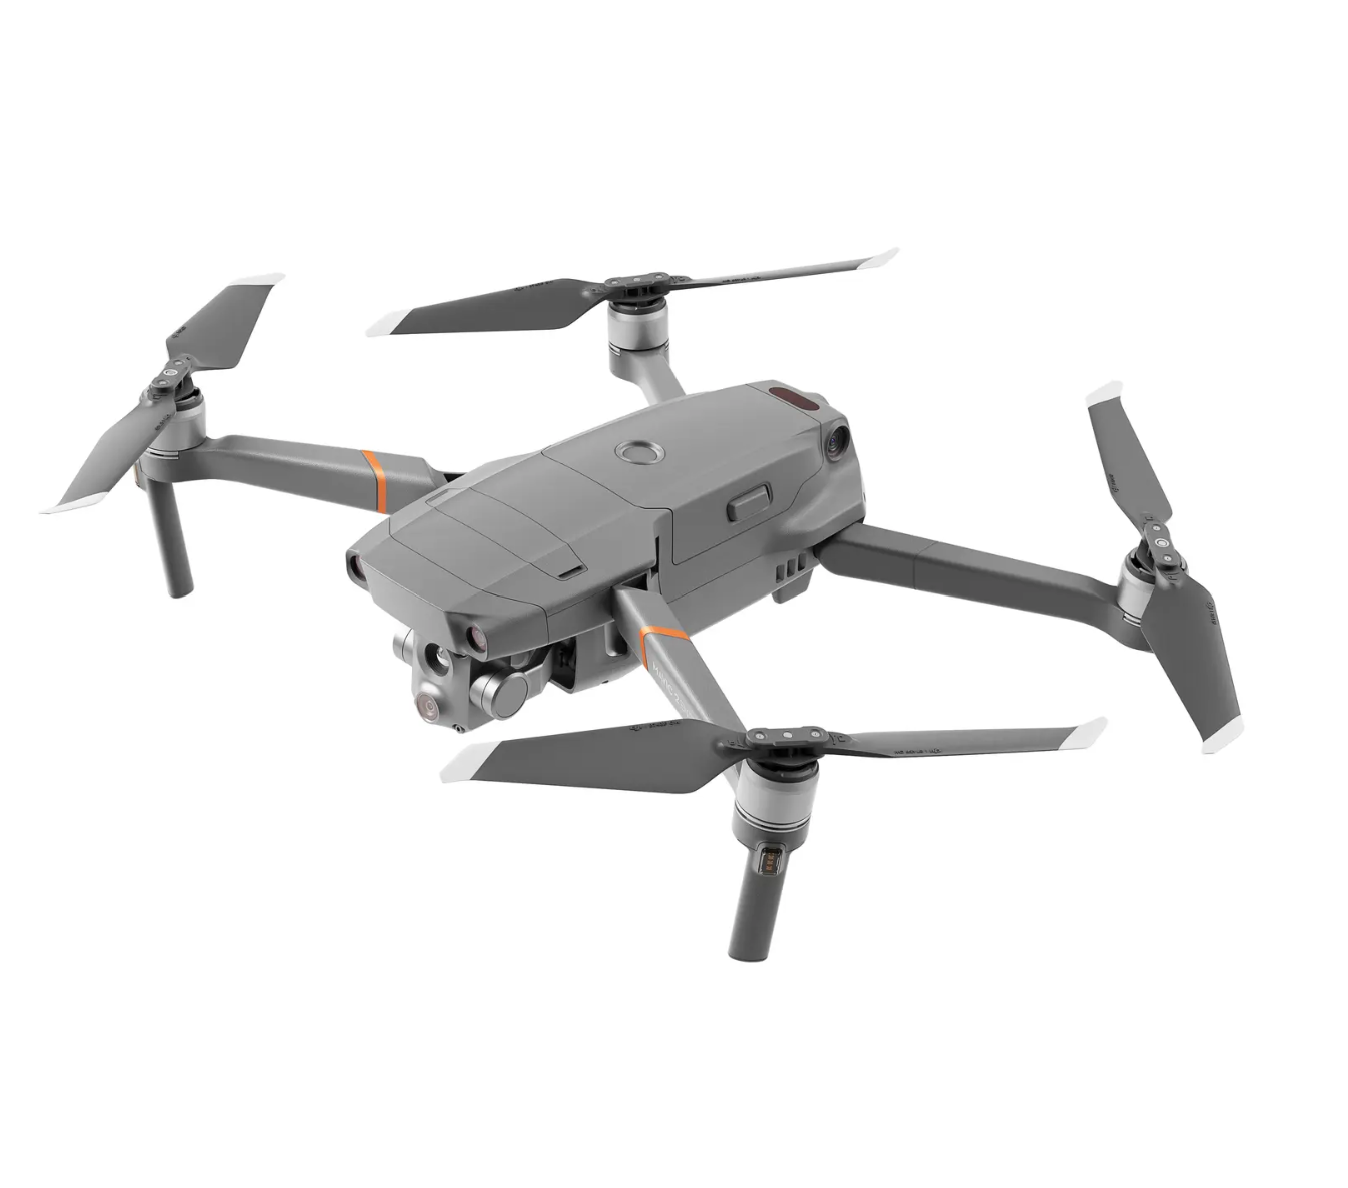
\includegraphics[width=0.65\textwidth,angle =0]{figure/DJI_mavick_2_enterprise.png}
\caption{Picture of the DJI Mavic 2 Enterprise}
\end{figure}


The unmanned aerial vehicle (UAV) utilized in this project is the DJI Mavic 2 Enterprise, developed by the Chinese technology company DJI. This UAV has garnered widespread popularity in the commercial and industrial community due to its compact design, advanced camera capabilities, and ease of use.

The Mavic 2 Enterprise is equipped with a 3-axis gimbal stabilized camera that can capture high-quality 4K video and 12MP photos. It features omnidirectional obstacle sensing and avoidance with sensors positioned on the front, back, bottom, and sides, as well as a GPS and magnetometer sensor, which allows the drone to maintain a stable hovering position.

%\textcolor{red}{Ska detta vara med? In order to control the drone, an RC is necessary, which communicates with the drone on 2.4GHz or 5.8GHz depending on the surroundings.}
A compatible smartphone with a designated application must be connected to the RC via an USB cable if a live feed from the drone is desired. DJI offers its own application that offers pilots a wide array of modes, settings, and options to customize and monitor the live feed from the drone. This application can be downloaded from either the App Store or Google Play. However, given the autonomous nature of this project, a bespoke application tailored specifically for this purpose had to be developed.

The Mavic 2 Enterprise has a maximum flight time of up to 31 minutes and a range of up to 8 kilometers, making it a versatile and effective tool for various applications. However, it is important to note that drone laws and regulations vary by country and region, and certain areas may require permits to fly beyond visual line of sight or certain distances. Therefore, strict adherence to local regulations and safety protocols is of paramount importance when operating the Mavic 2 Enterprise or any other UAV.



\subsection{Samsung A13} \label{Samsung}
\begin{figure}[h!]
\centering
 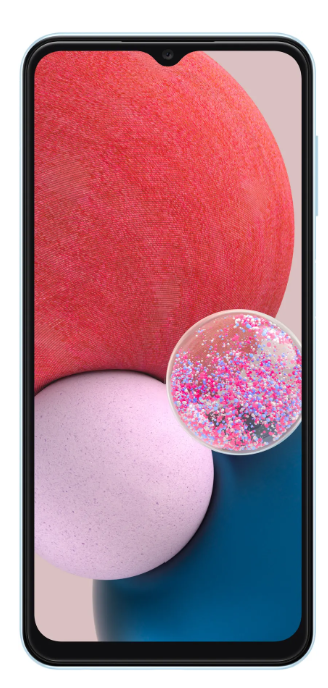
\includegraphics[width=0.25\textwidth,angle =90]{figure/Samsung_A13.png}
\caption{Picture of the Samsung A13}
\end{figure}
The device Samsung Galaxy A13 is an affordable and reliable mobile device with a long-lasting 5,000mAh battery.
In summary, the Samsung Galaxy A13 is a cost-effective and reliable mobile device that offers users a range of features and capabilities. Its robust hardware and user-friendly software make it a suitable choice for various applications, from basic computing tasks to multimedia editing and communication.



\section{Software} \label{Software}
This section will describe the software that is being used in this project, which is DJI Mobile SDK, ATOS, Android and Java.


\subsection{ISO DTS 22133 Communications Protocol} \label{ISO}
In order to properly test collision avoidance systems and carry out numerous other test, it is necessary to conduct testing on the specialized proving grounds, a controlled environment that is safe for both the driver and other motorists. In order to create realistic traffic scenarios, the proving grounds must make use of various targets that can represent both vehicles and / or pedestrians.

\begin{figure}[!h]
  \centering
  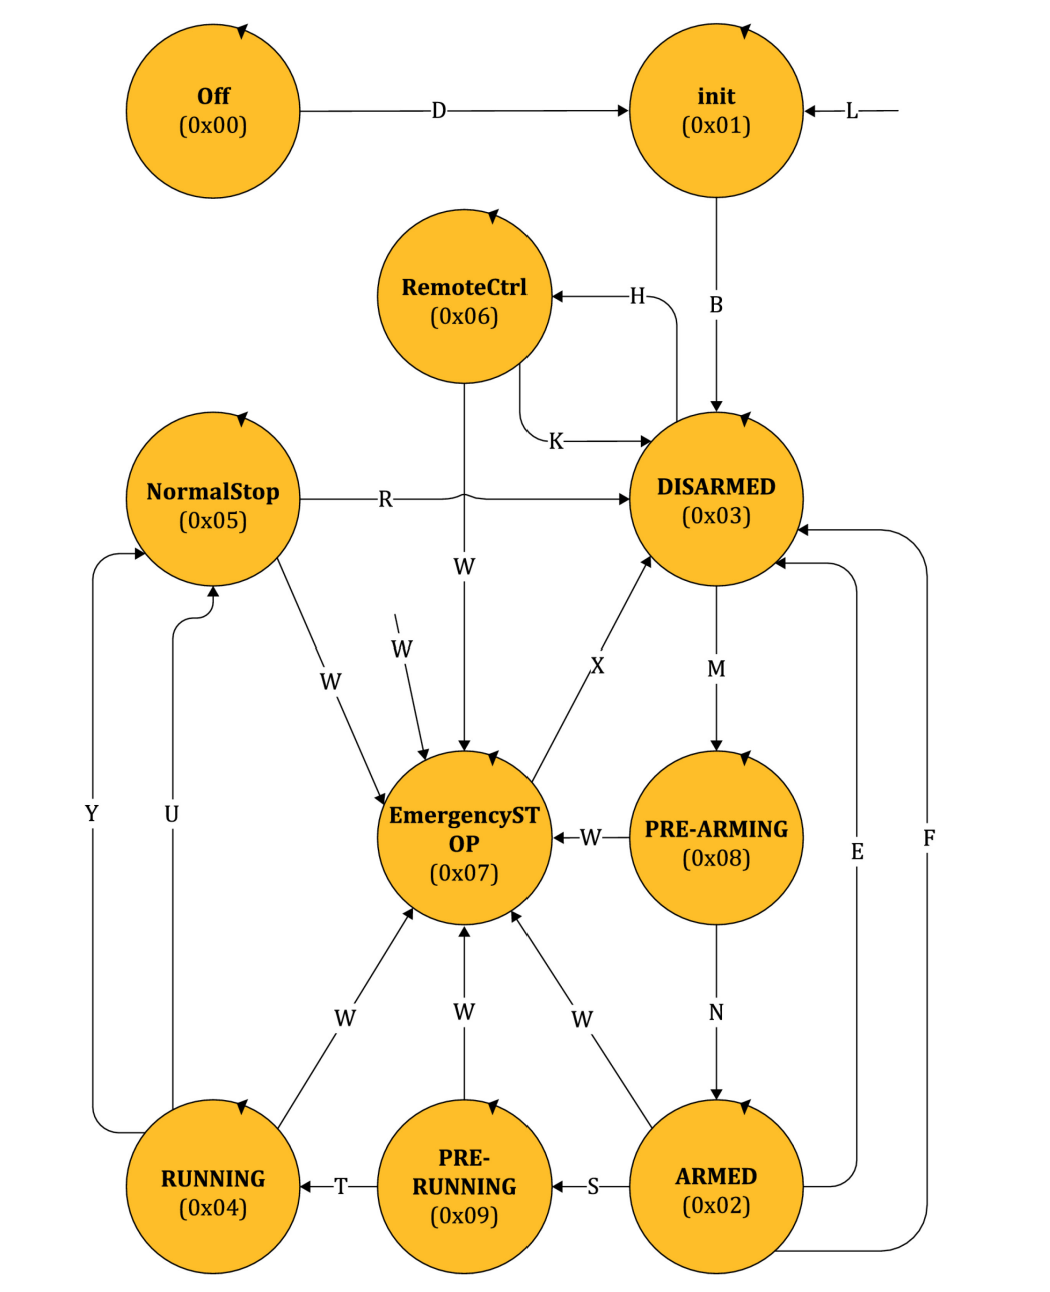
\includegraphics[scale=0.6]{figure/Olika_states.png}
  \caption{Test object states}
  \label{fig:iso_states}
\end{figure}

The ISO DTS 22133 document states the requirements, functionality, and protocol necessary for controlling multi target-carrier systems to create and monitor realistic traffic scenarios in a safe and effective manner.
The different states of the test object are displayed in figure~\ref{fig:iso_states}. The states are described in \ref{tab:states}

\begin{table}[!h]
  \centering
  \begin{tabular}{|c|c|p{0.45\textwidth}|}
    \hline
    \textbf{State ID} & \textbf{State name} & \textbf{State description} \\
    \hline
    0x00 & OFF& Test object turned off \\
    \hline
    0x01 & INIT& Test object in initializing phase, e.g. setting up supporting system\\
    \hline
   0x02 & ARMED &Test object ready to execute the test \\
    \hline
    0x03 & DISARMED & Test object connected to the control center(in this case ATOS) \\
    \hline
    0x04& RUNNING & Test scenario is executing  \\
    \hline
    0x05 & NORMAL\_STOP &Test scenario has been executed/finished \\
    \hline
      0x06 & REMOTECONTROL & Test object is manually driven by the control center or external remote control\\
    \hline
     0x07 &EMERGENCY\_STOP & Test object is currently emergency stopping\\
    \hline
      0x08 &PRE-ARMING& Test object is currently preparing for arm\\
    \hline
      0x09 & PRE-RUNNING &Test object is waiting for running or preparing for running \\
    \hline
  
  \end{tabular}
  \caption{Test object state description}
  \label{tab:states}
\end{table} 
\subsection{Autonomous Vehicle testing operating system (ATOS)} \label{ATOS}
The core of each test is ATOS, short for Automatic Vehicle Testing Operating System, which follows different standards developed by AstaZero and creates paths for each object that is part of the test. An extensive comprehension of the ATOS software needs to be obtained, this includes the functional requirements, software specifications and the communication protocol. The information can be obtained from the ISO22133 protocol \todo{\cite{} till ISO} as well as in the actual codebase \todo{ref till ATOS github}. The project is mainly written in the programming languages C and C++ and developed on and Linux platform. The integration of ATOS in this project is illustrated in Figure~\ref{fig:ATOS-flow}.

\begin{figure}[H]
  \centering
  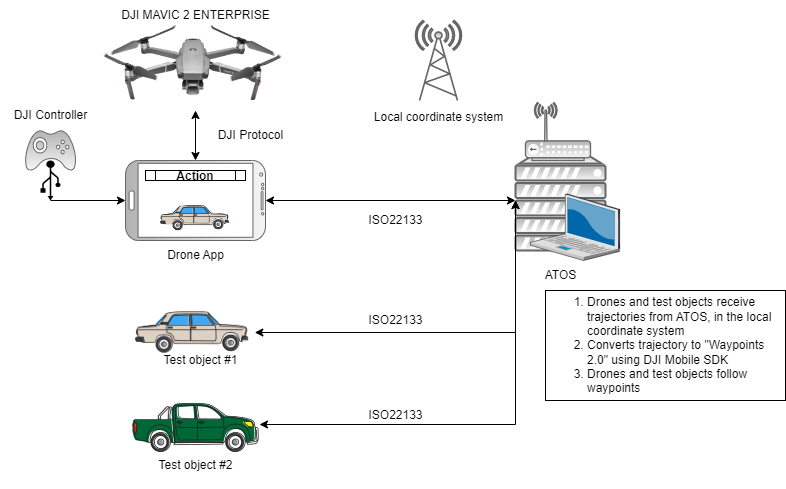
\includegraphics[width=\columnwidth]{figure/flow_config.png}
  \caption{ATOS integration with other objects}
  \label{fig:ATOS-flow}
\end{figure}




\subsection{Linux and Ubuntu 20.04} \label{Linux}
As stated in the last section, ATOS is being developed using a Linux operating system, specifically Ubuntu 20.04. Linux and Windows have some fundamental differences making it impossible to compile projects aimed at Linux operating systems on Windows. Both the ATOS project and the Android application provided by AstaZero have dependencies on other Linux programs which is why an old version of the Ubuntu operating system was required. The team therefore had to familiarize themselves with Ubuntu 20.04 and use it for all development purposes during the project. 

\subsection{Java, Android, SDKs and Android Studio} \label{Java, Android....}
The application is programmed in one of the major mobile operating systems named Android \todo{Ska de bara vara fakta här eller kan man skriva såhär?}. Android provides a framework for communicating with any mobile device running the Android operating system. The operating system is built using different activities which represent different parts of the application \todo{referens} and focuses on one single thing a user can do. For instance, one activity could be the landing page of the application while another activity could be the interface which communicates with the drone. Together these different activities makes up the application and communicate which each other.
\\ \\
The recommended option to develop Android applications is Android's own program called Android Studio. The program provides all necessary tools for developing Android applications in Java. It has also support for designing the user interface in both a visual studio and using the programming language XML.
\\ \\
Android enables the developers to use outside libraries, also called Software Development Kits (SDK). These external libraries allows the developer to use other code written by other developers and use their frameworks. DJI provides their own SDK for communicating with their different products.
\\ \\
\todo{Ska flytta om nästa stycke}
To access the functionalities of the DJI Mavic 2 Enterprise drone, a mobile application must be connected to the drone's remote controller (RC). As previously stated, DJI provides a framework for Android devices, which enables users to access functions such as reading drone states, initiating or terminating video recording, obtaining a live feed from the drone's camera, land at a given point and starting or stopping the motors. DJI's website contains tutorials on how to implement various types of functions for the application, which have served as a foundation for learning how to communicate with the drone in this study. Moreover, GitHub hosts a diverse range of projects of varying kinds that have been explored to acquire knowledge of the DJI Mobile SDK API.
Given that AstaZero provided an Android phone, the app-development was limited to Android.
\todo{Här behövs det skrivas mer om hur vi går tillväga för att få drönaren att bli "självkörande".}



\subsection{AstaZero's app} \label{AZ's app}
\todo{SKRIV}
\subsection{DJI Waypointmission}
\todo{SKRIV}



\subsection{Image tracking} \label{Image tracking}
In order to ensure that the camera capture the vehicles at the optimal angle, it was imperative for the drones to accurately detect the location of the cars as the drones followed them. Regarding research and implementation of object detection and image tracking, Tensorflow lite was used, which offered an extensive amount of documentation on the subject. Tensorflow lite offer a fast object detection response due to that Tensorflow models is compressed Tensorflow lite models. The output from this object detection will be an rectangle that cover the object, what the object is labeled as, the confidence for what the object is and lastly the index of the object.
\\ \\
Since Tensorflow lite only offers object detection and not object tracking, an algorithm to keep track of the objects needs to be applied. Which will make that the output of the object detection will go into the tracking algorithm before the application can send instructions wheter the gimbal should change the camera angel.

\subsection{Tracking Algorithm} \label{Tracking algorithm}
When keeping track of the objects the application needs to store the data from previous detection. Due to that the algorithm needs to keep track of where each object is and if a new object is in the image and also be able to confidently say that the previous object and this object is the same. 
\\ \\
A method that could be used in this algorithm is the Kalman filter \todo{kalman filter källa: https://reader.elsevier.com/reader/sd/pii/B9780128175880000106?token=FBA2F3B115B43B99DABD4E9FF292CBDFB4BA91B5D4FC3B463EC2900DD753433806C06C8E4EC57ED820C099F754E465BB&originRegion=eu-west-1&originCreation=20230504134811} which would predict the next location of the object by taking the acceleration, velocity and position into account. This would help since car is moving faster than the drone in most tests and by using the Kalman filter the car doesn't go too far away before the gimbal reacts.


\subsection{Graphical User Interface} \label{GUI}
Developing the GUI for the app includes designing an effective, functional and informative interface that is easy to use while also providing all the necessary controls for operating it and capturing the footage. Below are some scientifically based (GUIDELINES FOR DEVELOPING A GOOD GUI), as well as some project-based, considerations for GUI-development. 
\\

\begin{itemize}
    \item \textbf{Creating a user centered interface:} The GUI should be intuitive and easy to navigate. 
    \item \textbf{Include all necessary commands:} Evaluate what commands are needed for executing the program and make them easily accessible. 
    \item \textbf{Create a distinct visual hierarchy:} Prioritize important information and make it easy for the user to locate the necessary information. 
    \item \textbf{Real-time representation:} The GUI should provide users with the real-time footage captured by the drone as well as real time updates of the drones battery life etc. 
    
\end{itemize}


%% GUIDELINES FOR DEVELOPING A GOOD GUI,https://indico.cern.ch/event/0/contributions/1294438/attachments/747/1334/IA_CHEP04_paper.pdf








%\section{Equation}
%\begin{equation}
%f(t)=\left\{ \begin{array}{ll}
%1,~~~~ & t< 1 \\
%t^2 & t\geq 1
%\end{array}\right.
%\end{equation}

%\section{Table}
%\begin{table}[H]
%\centering
%\caption{Values of $f(t)$ for $t=0,1,\dots 5$.}
%\begin{tabular}{l|llllll} \hline\hline
%$t$ & 0 & 1 & 2 & 3 & 4 & 5 \\ \hline
%$f(t)$ & 1 & 1 & 4 & 9 & 16 & 25 \\ \hline\hline
%\end{tabular}
%\end{table}


%\section{List}
%\begin{enumerate}
%  \item The first item
%  \begin{enumerate}
%    \item Nested item 1
%    \item Nested item 2
%  \end{enumerate}
%  \item The second item
%  \item The third item 
%  \item \dots
%\end{enumerate}
The design of the app has as of yet not been finalized, however some early drafts have been developed. Due to the decision to start off by developing two applications later to be merged, one for image recognition and one for making the drone fly along a trajectory sent from the app, the first version of the app implemented these functions seperately. When launching this app the first step was connecting the app to the drone. When successfully connected you were given two choices, launching the image recognition application or the waypoint mission application which allowed the drone to follow a trajectory. These different applications were rather similar, most of the screen was covered by the video feed from the drone and had some buttons to control relevant drone functions in each application. Both of these early applications therefore accomplish the previously set goals, looks-wise they do however leave something to be desired. The final design of the app will be based on the design of the waypoint mission app. We have not decided on which actions the app will allow the user to take. Since the drone is controlled by both the app and ATOS, the different actions can be implemented in either ATOS or the app. ATOS being the brain of the testing and in charge of coordinating all vehicles partaking in a test, should control the more important actions like starting a test, but letting the user of the app control some actions could be beneficial. A stop-button to make the drone stop, a return-to-home button that makes the drone fly back to its starting position are examples of useful actions to be implemented in the app. 

The finer design choices such as color palette, what style of buttons to be used et cetera will be made when the functionality of the app is working as desired.


\section{Limitations} \label{Limitations}
This section will delineate the limitations associated with the utilization of the drone, WaypointMission, and the DJI SDK application.


\subsection{Drone limitations} \label{Dron limitations}
Research into drone capabilities and limitations was needed to obtain necessary information on the feasibility of achieving the performance requirements. Continuous communication with AstaZero was conducted regarding the implementation of the android app and drone software.

\subsection{Limits of WaypointMission} \label{limits of waypointmission}
\label{sec:limit_WP}
The software used to fly the drone missions, WaypointMission [Ref]\todo{referens}, had some limitations that limited how far a drone could fly while filming a test. The drone could only fly a mission with a radius of 500 meters or less. The current tests that this software aimed to film had a radius shorter than 500 meters and is therefore not a problem. If AstaZero wished to use this software to conduct other tests, this needs to be considered to ensure that the test would run.
\\ \\
WaypointMission also has a limit of 99 predetermined waypoints per mission. This creates a big limitation in how accurate the drone can be for larger missions and needs to be handled in the code. The trajectory sent over by ATOS might be larger than 99 points and needs to be reduced. \todo{Skriva mer och ska det ligga här?}
\todo{Skriva att man måste ladda upp missions innan, inte on the fly}

\subsection{Limits of DJI SDK} \label{limits of dji sdk}
By using DJI SDK ActiveTrackMission there is the possibility to detect and track a chosen object. But due to that DJI limit the use of multiple missions running simultaneously, ActiveTrackMission won't be able to run during the WaypointMission. Which leads to that the gimbal will be controlled and used through another tracking algorithm. \todo{ActiveTrack källa https://developer.dji.com/api-reference/android-api/Components/Missions/DJIActiveTrackMissionOperator.html}
\\ \\
When choosing another algorithm to use for object tracking there needs to be considered that the provided application by AstaZero is using an older android SDK version that most object detection programs want. Which will make the object detection options smaller due to that alternatives such as OpenCV and Google's ML-kit can't be supported.

\newpage

\section{Source code listing}
%\lstset{language=Matlab}
\begin{lstlisting}[frame=single]
% Generate x- and y-nodes
x=linspace(0,1); y=linspace(0,1);

% Calculate z=f(x,y)
for i=1:length(x)
 for j=1:length(y)
  z(i,j)=x(i)+2*y(j);
 end
end
\end{lstlisting}

%\section{To-do note}
%The \texttt{todo} package enables to-do notes to be added in the page margin. This can be a very convenient way of making notes in the document during the process of writing. All notes can be hidden by using the option \emph{disable} when loading the package in the settings. \todo{Example of a to-do note.}

